\chapter{Todennäköisyys}

Tässä luvussa tutustumme todennäköisyyslaskennan
perustekniikoihin, joita tarvitsee yleisimmin
kisakoodauksessa.
Todennäköisyyksien laskenta on pääasiassa
matematiikkaa, mutta usein mukana esiintyy
myös dynaamista ohjelmointia,
jotta todennäköisyyden saa laskettua tehokkaasti.

\section{Perusasiat}

Todennäköisyys on luku väliltä $0 \ldots 1$,
joka kuvaa sitä, miten todennäköinen jokin
tapahtuma on.
Varman tapahtuman todennäköisyys on 1,
ja mahdottoman tapahtuman todennäköisyys on 0.

Tyypillinen esimerkki todennäköisyydestä
on nopan heitto, jossa tuloksena
on silmäluku väliltä $1,2,\ldots,6$.
Yleensä oletetaan, että kunkin silmäluvun
todennäköisyys on $1/6$
eli kaikki tulokset ovat yhtä todennäköisiä.

Tapahtuman todennäköisyyttä merkitään $P(\cdots)$,
jossa kolmen pisteen tilalla on tapahtuman kuvaus.
Esimerkiksi nopan heitossa
$P(\textrm{''silmäluku on 4''})=1/6$,
$P(\textrm{''silmäluku ei ole 6''})=5/6$
ja $P(\textrm{''silmäluku on parillinen''})=1/2$.

\subsection{Laskutavat}

Tapahtuman todennäköisyyden laskemiseen on
kaksi tavallista laskutapaa. Tutustumme niihin
seuraavan tehtävän avulla:

\begin{task}
Korttipakassa on 52 korttia, jotka jakaantuvat
neljään maahan (hertta, risti, ruutu, pata).
Kussakin maassa on 13 korttia, joiden arvot ovat $1,2,\ldots,13$.
Sinulle jaetaan kolme korttia pakasta.
Mikä on todennäköisyys, että jokaisen kortin arvo on sama?
\end{task}

\subsubsection*{Laskutapa 1}

Kombinatorisessa laskutavassa
todennäköisyyden kaava on

\[\frac{\textrm{halutut tapaukset}}{\textrm{kaikki tapaukset}}.\]

Tässä tehtävässä halutut tapaukset ovat niitä,
joissa jokaisen kolmen kortin arvo on sama.
Tällaisia tapauksia on $13 {4 \choose 3}$,
koska on 13 vaihtoehtoa, mikä on kortin arvo,
ja ${4 \choose 3}$ tapaa valita 3 maata 4 mahdollisesta.

Kaikkien tapausten määrä on ${52 \choose 3}$,
koska 52 kortista valitaan 3 korttia.
Niinpä tapahtuman todennäköisyys on

\[\frac{13 {4 \choose 3}}{{52 \choose 3}} = \frac{1}{425}.\]

\subsubsection*{Laskutapa 2}

Toinen tapa laskea todennäköisyys on simuloida prosessia,
jossa tapahtuma syntyy.
Tässä tapauksessa pakasta nostetaan kolme korttia,
joten prosessissa on kolme vaihetta.
Vaatimuksena on, että prosessin jokainen vaihe onnistuu.

Ensimmäisen kortin nosto onnistuu varmasti,
koska mikä tahansa kortti kelpaa.
Tämän jälkeen kahden seuraavan kortin
arvon tulee olla sama.
Toisen kortin nostossa kortteja on jäljellä 51
ja niistä 3 kelpaa, joten todennäköisyys on $3/51$.
Vastaavasti kolmannen kortin nostossa
todennäköisyys on $2/50$.

Todennäköisyys koko prosessin onnistumiselle on

\[1 \cdot \frac{3}{51} \cdot \frac{2}{50} = \frac{1}{425}.\]

\subsection{Tapahtumat}

Todennäköisyyden tapahtuma voidaan tulkita
joukkona, joka sisältää alkeistapauksia.
Esimerkiksi nopan heitossa alkeistapaukset
ovat $\{1,2,\ldots,6\}$, missä kukin
alkeistapaus vastaa silmälukua
ja sen todennäköisyys on $1/6$.

Esimerkiksi joukko $A=\{2,4,6\}$
vastaa tapahtumaa ''silmäluku on parillinen''
ja joukko $B=\{1,2,3,4\}$ vastaa tapahtumaa
''silmäluku on alle 5''.
Tapahtumien todennäköisyydet ovat $P(A)=1/2$
ja $P(B)=2/3$.

Komplementti $\bar A$
tarkoittaa tapahtumaa ''$A$ ei tapahdu''.
Yhdiste $A \cup B$
tarkoittaa ''$A$ tai $B$ tapahtuu'',
ja leikkaus
$A \cap B$ tarkoittaa
''$A$ ja $B$ tapahtuvat''.

\subsubsection*{Komplementti}

Komplementin $\bar A$
todennäköisyys lasketaan $P(\bar A)=1-P(A)$.
Joskus tehtävän ratkaisu on kätevää
laskea komplementin kautta.
Esimerkiksi todennäköisyys saada
10 nopan heitossa ainakin
kerran silmäluku 6 on $1-(5/6)^{10}$,
missä $5/6$ on todennäköisyys, että silmäluku ei ole 6.

\subsubsection*{Yhdiste}

Yhdisteen $A \cup B$ todennäköisyys lasketaan kaavalla 

\[P(A \cup B)=P(A)+P(B)-P(A \cap B).\]

Esimerkiksi jos $A=\textrm{''silmäluku on parillinen''}$
ja $B=\textrm{''silmäluku on alle 5''}$,
niin tapahtuman $A \cup B$ todennäköisyys
on $P(A)+P(B)-P(A \cap B)=1/2+2/3-1/3=5/6$.
Joukko $A \cup B$ sisältää tapaukset $\{1,2,3,4,6\}$.

Jos tapahtumat $A$ ja $B$ ovat erilliset eli $A \cap B$ on tyhjä,
yhdisteen $A \cup B$ todennäköisyys on yksinkertaisesti

\[P(A \cup B)=P(A)+P(B).\]

\subsubsection*{Leikkaus}

Leikkauksen $A \cap B$ todennäköisyys lasketaan kaavalla

\[P(A \cap B)=P(A)P(B|A),\]

missä $P(B|A)$ on $B$:n todennäköisyys
ehdolla, että $A$ on tapahtunut.

Esimerkiksi jos $A=\textrm{''silmäluku on parillinen''}$
ja $B=\textrm{''silmäluku ei ole 6''}$,
niin tapahtuman $A \cap B$ todennäköisyys
on $P(A)P(B|A)=1/2 \cdot 2/3 = 1/3$.
Joukko $A \cap B$ sisältää tapaukset $\{2,4\}$.


Jos tapahtumat $A$ ja $B$ ovat riippumattomat
eli $A$:n tapahtuminen ei vaikuta $B$:n todennäköisyyteen
ja päinvastoin, leikkauksen todennäköisyys on

\[P(A \cap B)=P(A)P(B),\]

koska tässä tapauksessa $P(B|A)=P(B)$.

\section{Satunnaismuuttuja}

Satunnaismuuttuja on arvo, joka syntyy satunnaisen
prosessin tuloksena.
Satunnaismuuttujaa merkitään yleensä
suurella kirjaimella.
Kahden nopan heitossa yksi mahdollinen
satunnaismuuttuja on $X=\textrm{''silmälukujen summa''}$.
Esimerkiksi jos heitot ovat $[4,6]$,
niin $X$ saa arvon 10.

Merkintä $P(X=x)$ tarkoittaa todennäköisyyttä,
että satunnaismuuttujan $X$ arvo on $x$.
Edellisessä esimerkissä $P(X=10)=3/36$,
koska erilaisia heittotapoja on 36
ja niistä summan 10 tuottavat heitot
$[4,6]$, $[5,5]$ ja $[6,4]$.

\subsection{Odotusarvo}

Odotusarvo $E[X]$ kertoo, mikä satunnaismuuttujan $X$
arvo on keskimääräisessä tilanteessa.
Odotusarvo lasketaan summana

\[\sum_x P(X=x)x,\]

missä $x$ saa kaikki mahdolliset satunnaismuuttujan arvot.

Esimerkiksi yhden nopan heitossa silmäluvun odotusarvo
on $1/6 \cdot 1 + 1/6 \cdot 2 + 1/6 \cdot 3 + 1/6 \cdot 4 + 1/6 \cdot 5 + 1/6 \cdot 6 = 7/2$.

\subsubsection*{Lineaarisuus}

Usein hyödyllinen odotusarvon ominaisuus on \textit{lineaarisuus}.
Sen ansiosta summa $E[X_1+X_2+\cdots+X_n]$ voidaan laskea $E[X_1]+E[X_2]+\cdots+E[X_n]$.
Kaava pätee myös silloin, kun satunnaismuuttujat riippuvat toisistaan.

Esimerkiksi kahden nopan heitossa silmälukujen summan odotusarvo on
$E[X_1+X_2]=E[X_1]+E[X_2]=7/2+7/2=7$.

Seuraava tehtävä on hieman vaativampi:

\begin{task}
Pöydällä on $n$ hattua ja $n$ palloa.
Jokainen pallo sijoitetaan satunnaisesti johonkin hattuun.
Mikä on odotusarvo, montako hattua on tyhjiä?
\end{task}

Todennäköisyys, että yksittäinen hattu on tyhjä,
on $(\frac{n-1}{n})^n$, koska mikään pallo ei saa mennä sinne.
Odotusarvon lineaarisuuden ansiosta tyhjien hattujen
määrän odotusarvo on $n \cdot (\frac{n-1}{n})^n$.

\subsection{Jakaumat}

Satunnaismuuttujan jakauma kertoo,
millä todennäköisyydellä satunnaismuuttuja
saa minkäkin arvon.
Jakauma muodostuu arvoista $P(X=x)$.
Esimerkiksi kahden nopan heitossa
silmälukujen summan jakauma on:
\begin{center}
\small {
\begin{tabular}{r|rrrrrrrrrrrrr}
$x$ & 2 & 3 & 4 & 5 & 6 & 7 & 8 & 9 & 10 & 11 & 12 \\
$P(X=x)$ & $1/36$ & $2/36$ & $3/36$ & $4/36$ & $5/36$ & $6/36$ & $5/36$ & $4/36$ & $3/36$ & $2/36$ & $1/36$ \\
\end{tabular}
}
\end{center}
Tutustumme seuraavaksi muutamaan usein esiintyvään jakaumaan.

\subsubsection*{Tasajakauma}

Tasajakaumassa satunnaismuuttuja
saa arvoja väliltä $a \ldots b$
ja jokaisen arvon todennäköisyys on sama.
Esimerkiksi yhden nopan heitto tuottaa tasajakauman,
jossa $P(X=x)=1/6$, kun $x=1,2,\ldots,6$.

Tasajakaumassa $X$:n odotusarvo on
\[E[X] = \frac{a+b}{2}.\]

\subsubsection*{Binomijakauma}

Binomijakauma kuvaa tilannetta, jossa tehdään $n$
yritystä ja joka yrityksessä onnistumisen
todennäköisyys on $p$. Satunnaismuuttuja $X$
on onnistuneiden yritysten määrä.

Satunnaismuuttujan arvon $x$ todennäköisyys on

\[P(X=x)=p^x (1-p)^{n-x} {n \choose x},\]

missä $p^x$ kuvaa onnistuneita yrityksiä,
$(1-p)^{n-x}$ kuvaa epäonnistuneita yrityksiä
ja ${n \choose x}$ antaa erilaiset tavat,
miten yritykset sijoittuvat toisiinsa nähden.

Esimerkiksi jos heitetään 10 kertaa noppaa,
todennäköisyys saada tarkalleen 3 kertaa silmäluku 6
on $(1/6)^3 (5/6)^7 {10 \choose 3}$.

Binomijakaumassa $X$:n odotusarvo on
\[E[X] = pn.\]

\subsubsection*{Geometrinen jakauma}

Geometrinen jakauma kuvaa tilannetta,
jossa onnistumisen todennäköisyys on $p$
ja yrityksiä tehdään, kunnes tulee ensimmäinen
onnistuminen. Satunnaismuuttuja $X$ on
tarvittavien heittojen määrä.

Satunnaismuuttujan arvon $x$ todennäköisyys on

\[P(X=x)=(1-p)^{x-1} p,\]

missä $(1-p)^{x-1}$ kuvaa epäonnistuneita yrityksiä ja
$p$ on ensimmäinen onnistunut yritys.

Esimerkiksi jos heitetään noppaa,
kunnes tulee silmäluku 6, todennäköisyys
heittää tarkalleen 4 kertaa on $(5/6)^3 1/6$.

Geometrisessa jakaumassa $X$:n odotusarvo on
\[E[X]=\frac{1}{p}.\]

\section{Markovin ketju}

Markovin ketju on satunnaisprosessi,
joka muodostuu tiloista ja niiden välisistä siirtymistä.
Jokaisesta tilasta tiedetään, millä todennäköisyydellä
siitä siirrytään toisiin tiloihin.
Luonteva tapa esittää Markovin ketju on
muodostaa verkko, jonka solmut ovat tiloja
ja kaaret niiden välisiä siirtymiä.

\begin{task}
Rakennuksessa on $n$ kerrosta.
Aloitat kerroksesta 1 ja liikut joka askeleella
satunnaisesti kerroksen ylöspäin tai alaspäin.
Poikkeuksena kerroksesta 1 liikut aina ylöspäin
ja kerroksesta $n$ aina alaspäin.
Mikä on todennäköisyys, että olet $m$
askeleen jälkeen kerroksessa $k$?
\end{task}

Tehtävässä kukin rakennuksen kerros
on yksi tiloista, ja kerrosten välillä liikutaan
satunnaisesti.
Esimerkiksi jos $n=5$, verkosta tulee:

\begin{center}
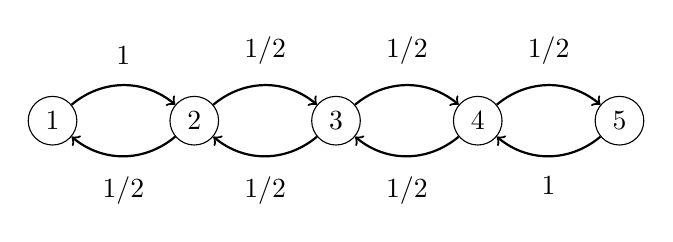
\begin{tikzpicture}[scale=0.9]
\node[draw, circle] (1) at (0,0) {$1$};
\node[draw, circle] (2) at (2,0) {$2$};
\node[draw, circle] (3) at (4,0) {$3$};
\node[draw, circle] (4) at (6,0) {$4$};
\node[draw, circle] (5) at (8,0) {$5$};

\path[draw,thick,->] (1) edge [bend left=40] node[font=\small,label=$1$] {} (2);
\path[draw,thick,->] (2) edge [bend left=40] node[font=\small,label=$1/2$] {} (3);
\path[draw,thick,->] (3) edge [bend left=40] node[font=\small,label=$1/2$] {} (4);
\path[draw,thick,->] (4) edge [bend left=40] node[font=\small,label=$1/2$] {} (5);

\path[draw,thick,->] (5) edge [bend left=40] node[font=\small,label=below:$1$] {} (4);
\path[draw,thick,->] (4) edge [bend left=40] node[font=\small,label=below:$1/2$] {} (3);
\path[draw,thick,->] (3) edge [bend left=40] node[font=\small,label=below:$1/2$] {} (2);
\path[draw,thick,->] (2) edge [bend left=40] node[font=\small,label=below:$1/2$] {} (1);

%\path[draw,thick,->] (1) edge [bend left=40] node[font=\small,label=below:$1$] {} (2);
\end{tikzpicture}
\end{center}

Markovin ketjun tilajakauma on vektori
$[p_1,p_2,\ldots,p_n]$, missä $p_k$ tarkoittaa
todennäköisyyttä olla tällä hetkellä tilassa $k$.
Todennäköisyyksille pätee aina $p_1+p_2+\cdots+p_n=1$.

Esimerkissä jakauma on ensin $[1,0,0,0,0]$,
koska on varmaa, että kulku alkaa kerroksesta 1.
Seuraava jakauma on $[0,1,0,0,0]$,
koska kerroksesta 1 pääsee vain kerrokseen 2.
Tämän jälkeen on mahdollisuus mennä joko ylöspäin
tai alaspäin, joten seuraava jakauma on $[1/2,0,1/2,0,0]$ jne.

Tehokas tapa simuloida kulkua Markovin ketjussa
on käyttää dynaamista ohjelmointia.
Ideana on pitää yllä tilajakaumaa
ja käydä joka vuorolla läpi kaikki tilat
ja jokaisesta tilasta kaikki mahdollisuudet jatkaa eteenpäin.

Markovin ketjun tilasiirtymät voi esittää myös matriisina,
jonka avulla voi päivittää tilajakaumaa askeleen eteenpäin.
Tässä tapauksessa matriisi on

\[ 
 \begin{bmatrix}
  0 & 1/2 & 0 & 0 & 0 \\
  1 & 0 & 1/2 & 0 & 0 \\
  0 & 1/2 & 0 & 1/2 & 0 \\
  0 & 0 & 1/2 & 0 & 1 \\
  0 & 0 & 0 & 1/2 & 0 \\
 \end{bmatrix}.
\]

Ideana on, että matriisilla voi kertoa tilajakaumaa esittävän
vektorin, jolloin saadaan seuraava tilajakauma.
Esimerkiksi jakaumasta $[1,0,0,0,0]$ pääsee jakaumaan
$[0,1,0,0,0]$ seuraavasti:

\[ 
 \begin{bmatrix}
  0 & 1/2 & 0 & 0 & 0 \\
  1 & 0 & 1/2 & 0 & 0 \\
  0 & 1/2 & 0 & 1/2 & 0 \\
  0 & 0 & 1/2 & 0 & 1 \\
  0 & 0 & 0 & 1/2 & 0 \\
 \end{bmatrix}
 \begin{bmatrix}
  1 \\
  0 \\
  0 \\
  0 \\
  0 \\
 \end{bmatrix}
=
 \begin{bmatrix}
  0 \\
  1 \\
  0 \\
  0 \\
  0 \\
 \end{bmatrix}.
\]

Tähän matriisiin voi soveltaa edelleen tehokasta
matriisipotenssia, jonka avulla voi laskea nopeasti,
mikä on jakauma $m$ askeleen jälkeen.

\section{Satunnaisalgoritmit}

Joskus tehtävässä voi hyödyntää satunnaisuutta,
vaikka tehtävä ei itsessään liittyisi todennäköisyyteen.
Satunnaisalgoritmit ovat algoritmeja, joiden toiminta
perustuu satunnaisuuteen.

\textit{Monte Carlo -algoritmi} on satunnaisalgoritmi,
joka saattaa tuottaa joskus väärän vastauksen.
Jotta algoritmi olisi käyttökelpoinen,
väärän vastauksen todennäköisyyden tulee olla pieni.

\textit{Las Vegas -algoritmi} on satunnaisalgoritmi,
joka tuottaa aina oikean tuloksen mutta jonka
suoritusaika vaihtelee satunnaisesti.
Tavoitteena on, että algoritmi toimisi nopeasti
suurella todennäköisyydellä.

\subsection{Alkion etsiminen}

\begin{task}
Annettuna on taulukko, jossa on $n$ alkiota.
Tehtäväsi on selvittää, mikä alkio on järjestetyssä
taulukossa kohdassa $k$.
\end{task}

Helppo ratkaisu tehtävään on järjestää
taulukko ajassa $O(n \log n)$, minkä jälkeen
haluttu alkio on kohdassa $k$.
Mutta onko tarpeen järjestää koko taulukkoa
yhden alkion selvittämiseksi?

Osoittautuu, että tehtävän voi ratkaista myös
satunnaisalgoritmilla.
Algoritmi on Las Vegas -tyyppinen:
sen aikavaativuus on yleensä $O(n)$,
mutta pahimmassa tapauksessa $O(n^2)$.

Ideana on valita taulukosta satunnainen alkio $x$
ja siirtää $x$:ää pienemmät alkiot
taulukon vasempaan osaan ja loput alkiot
taulukon oikeaan osaan.
Tämä vie aikaa $O(n)$, kun taulukossa on $n$ alkiota.
Oletetaan, että vasemmassa osassa on $a$
alkiota ja oikeassa osassa on $b$ alkiota.

Nyt jos $a=k-1$, alkio $x$ on haluttu alkio.
Jos $a>k-1$, etsitään rekursiivisesti
vasemmasta osasta, mikä on kohdassa $k$ oleva alkio.
Jos taas $a<k-1$, etsitään rekursiivisesti
oikeasta osasta, mikä on kohdassa $k-1-a$ oleva alkio.
Haku jatkuu vastaavasti, kunnes alkio on löytynyt.

Koska jokainen alkion $x$:n valinta
suunnilleen puolittaa taulukon,
alkion etsiminen vie aikaa $n+n/2+n/4+n/8+\cdots=O(n)$.

Algoritmin pahin tapaus on silti $O(n^2)$,
koska on mahdollista,
että $x$ valitaan sattumalta aina niin,
että se on taulukon pienin alkio.
Silloin taulukko pienenee joka vaiheessa
vain yhden alkion verran.
Tämän todennäköisyys on kuitenkin erittäin pieni,
eikä näin tapahdu koskaan käytännössä.

\subsection{Matriisitulon tarkastaminen}

\begin{task}
Annettuna on kolme $n \times n$ -kokoista matriisia
$A$, $B$ ja $C$.
Tehtäväsi on selvittää, päteekö $AB=C$.
\end{task}

Tehtävän voi ratkaista laskemalla matriisitulon
$AB$ ja tarkastamalla, onko se sama kuin $C$.
Matriisitulon laskemiseen menee aikaa
$O(n^3)$ perusalgoritmilla, mutta voisi toivoa,
että ratkaisun tarkastaminen olisi helpompaa
kuin sen laskeminen alusta alkaen uudestaan.

Tehtävän voi ratkaista Monte Carlo -algoritmilla,
jonka aikavaativuus on vain $O(n^2)$.
Idea on yksinkertainen: valitaan satunnainen
$n \times 1$ -matriisi $X$ ja lasketaan
matriisit $ABX$ ja $CX$.
Jos $ABX=CX$, ilmoitetaan, että $AB=C$,
ja muuten ilmoitetaan, että $AB \neq C$.

Algoritmin aikavaativuus on $O(n^2)$,
koska matriisien $ABX$ ja $CX$ laskeminen
vie aikaa $O(n^2)$.
Matriisin $ABX$ tapauksessa laskennan
voi suorittaa osissa $A(BX)$, jolloin riittää
kertoa kahdesti $n \times n$- ja $n \times 1$-kokoiset
matriisit.

Algoritmin heikkoutena on, että on pieni mahdollisuus,
että algoritmi erehtyy, kun se ilmoittaa, että $AB=C$.
Esimerkiksi 
\[
 \begin{bmatrix}
  2 & 4 \\
  1 & 6 \\
 \end{bmatrix}
\neq
 \begin{bmatrix}
  0 & 5 \\
  7 & 4 \\
 \end{bmatrix},
\]
mutta
\[
 \begin{bmatrix}
  2 & 4 \\
  1 & 6 \\
 \end{bmatrix}
 \begin{bmatrix}
  1 \\
  3 \\
 \end{bmatrix}
=
 \begin{bmatrix}
  0 & 5 \\
  7 & 4 \\
 \end{bmatrix}
 \begin{bmatrix}
  1 \\
  3 \\
 \end{bmatrix}.
\]
Käytännössä tämän todennäköisyys on kuitenkin hyvin
pieni ja tarvittaessa tarkastuksen voi tehdä usealla
satunnaisella matriisilla $X$ ennen vastauksen
$AB=C$ ilmoittamista.

\subsection{Verkon värittäminen}

\begin{task}
Annettuna on verkko, jossa on $n$ solmua ja $m$ kaarta.
Etsi tapa värittää verkon solmut kahdella värillä
niin, että ainakin $\lfloor m/2 \rfloor$ kaaressa
päätesolmut ovat eri väriset.
\end{task}

Esimerkiksi verkossa
\begin{center}
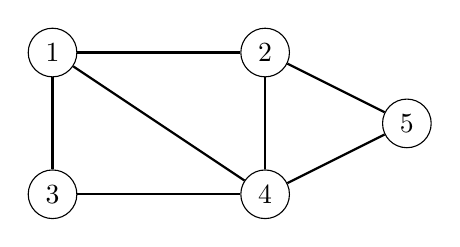
\begin{tikzpicture}[scale=0.9]
\node[draw, circle] (1) at (1,3) {$1$};
\node[draw, circle] (2) at (4,3) {$2$};
\node[draw, circle] (3) at (1,1) {$3$};
\node[draw, circle] (4) at (4,1) {$4$};
\node[draw, circle] (5) at (6,2) {$5$};

\path[draw,thick,-] (1) -- (2);
\path[draw,thick,-] (1) -- (3);
\path[draw,thick,-] (1) -- (4);
\path[draw,thick,-] (3) -- (4);
\path[draw,thick,-] (2) -- (4);
\path[draw,thick,-] (2) -- (5);
\path[draw,thick,-] (4) -- (5);
\end{tikzpicture}
\end{center}
yksi kelvollinen väritys on seuraava:
\begin{center}
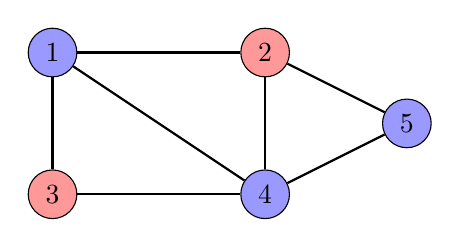
\begin{tikzpicture}[scale=0.9]
\node[draw, circle, fill=blue!40] (1) at (1,3) {$1$};
\node[draw, circle, fill=red!40] (2) at (4,3) {$2$};
\node[draw, circle, fill=red!40] (3) at (1,1) {$3$};
\node[draw, circle, fill=blue!40] (4) at (4,1) {$4$};
\node[draw, circle, fill=blue!40] (5) at (6,2) {$5$};

\path[draw,thick,-] (1) -- (2);
\path[draw,thick,-] (1) -- (3);
\path[draw,thick,-] (1) -- (4);
\path[draw,thick,-] (3) -- (4);
\path[draw,thick,-] (2) -- (4);
\path[draw,thick,-] (2) -- (5);
\path[draw,thick,-] (4) -- (5);
\end{tikzpicture}
\end{center}
Yllä olevassa verkossa on 7 kaarta ja niistä 5:ssä
päätesolmut ovat eri väriset,
joten väritys on kelvollinen.

Tehtävä on mahdollista ratkaista satunnaisalgoritmilla
muodostamalla satunnaisia värityksiä niin kauan,
kunnes syntyy kelvollinen väritys.
Satunnaisessa värityksessä jokaisen solmun väri on
valittu toisistaan riippumatta niin,
että kummankin värin todennäköisyys on $1/2$.

Satunnaisessa värityksessä todennäköisyys, että yksittäisen kaaren päätesolmut
ovat eri väriset on $1/2$. Niinpä odotusarvo, monessako kaaressa
päätesolmut ovat eri väriset, on $1/2 \cdot m \ge \lfloor m/2 \rfloor$.

Koska satunnainen väritys on odotusarvoisesti kelvollinen,
jokin kelvollinen väritys löytyy käytännössä nopeasti
muodostamalla satunnaisia värityksiä.